\subsection{Logiciel d'administration}
\par Il existe un bon nombre de logiciel d'administration pour cassandra, la pluspart propulsés par des communautés opensources.
\par Le logiciel retenu pour réaliser ce TP est la dernière version (\textit{1.3.1}) de DevCenter édité par \textcolor{cyan}{DataStax}.
Contrairement à d'autres logiciels essayés (OpsCenter, helenos) DevCenter est un client lourd, on n'y accède pas par
un navigateur web. Il ne sera donc pas installé sur le serveur mais sur notre ordinateur personnel. On ouvre en suite
une connection vers le Cleusteur.
\begin{block}{téléchargement}
\href{http://www.datastax.com/download-ops-dev}{http://www.datastax.com/download-ops-dev}
\end{block}

\begin{figure}[h!]
\centering
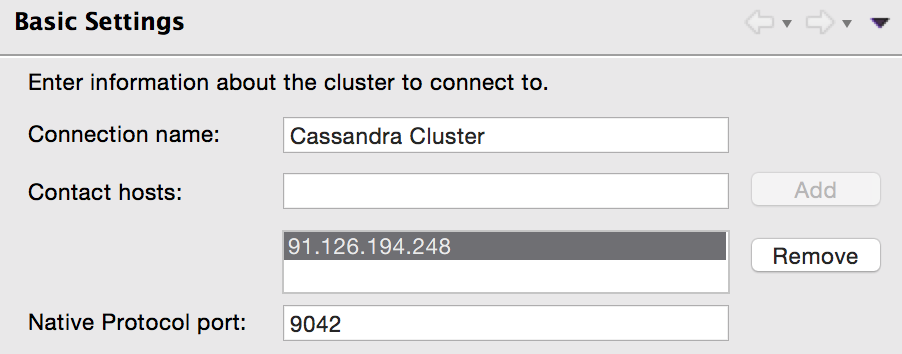
\includegraphics[scale=0.5]{img/ip.png}
\caption{Ajout du serveur sur le quel tourne Cassandra.}
\end{figure}

\par Une fois le logiciel installé et la connection enregistrée (figure 1.) on demande à Cassandra d'accepter les connections à 
distance, les \lq remote connections \rq. Pour cela on édite de nouveu le fichier \textit{casssandra.yaml}.
\begin{itemize}
\item \textcolor{cyan}{rpc\_address}\textcolor{magenta}{:} 0.0.0.0 (Anciennement localhost)
\item \textcolor{cyan}{broadcast\_rpc\_address}\textcolor{magenta}{:} 1.2.3.4
\end{itemize}

\par Une fois le tout configuré il est possible d'accéder à l'ensemble des keyspaces. Et de réaliser des requêtes sur la base.
Nour reviendrons sur cette interface pour illustrer des différents points du TP.
\begin{figure}[h!]
\centering
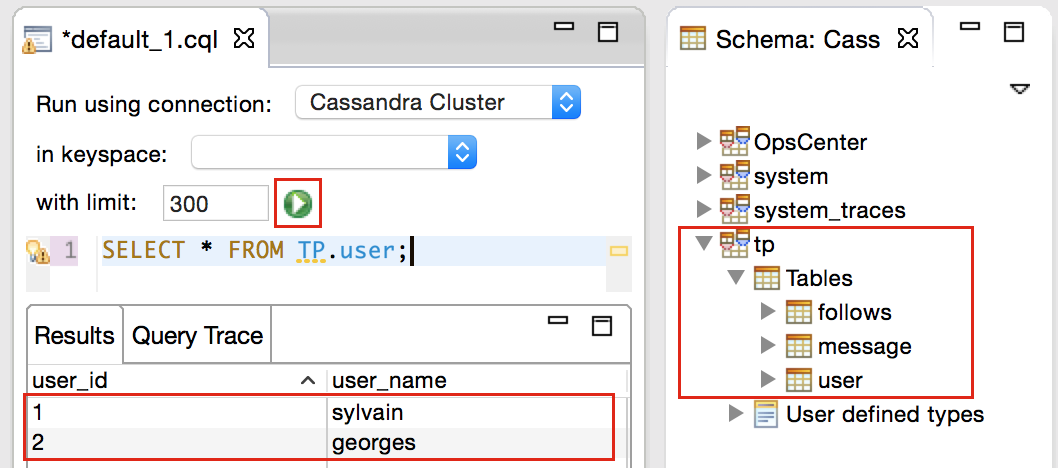
\includegraphics[scale=0.5]{img/select.png}
\caption{Exemple d'interface DevCenter par DataStax.}
\end{figure}